\section{Introduction}

One of the most recent challenges in cybersecurity systems is to outsource programs to be executed in the cloud maintaining the privacy of the owner and the security of data at the same time. The program code has to be protected alongside the data which is being used by it. Even in a securely encrypted code, the low-level instructions are visible when they are being executed by the CPU and a malicious operating system kernel can tamper with them. Several attacks are possible by reverse engineering the instructions, including code reuse, data injection, copyright violation, and recovery of classified data. Intel SGX (Software Guard eXtensions) \cite{sgx} is a novel architecture introduced with Intel Skylake micro-architecture \cite{skylake} that protects the code and the data inside an encrypted enclave that is a portion of memory protected by the support of hardware. The enclave is secure against direct eavesdropping by the adversary, but several successful attacking methods using side-channel information exist becuase  this information are visible to the adversary \cite{leakycauldron}. The main drawback of this hardware extension is that the memory layout is still visible to the operating system kernel. Therefore, a malicious OS in the cloud can recover useful information by observing the occurrences of page faults. As a result, this side-channel attack can be successful on recovering the data by clearing the page table and causing page faults, then observing them for different inputs. In the same scenario, cache-misses are a point for side-channel attacks. The pattern of cache-miss occurrences can be used by a malicious operating system to attack the enclave program.

Several theoretical and practical attacks based on SGX side channels are discussed and experimented to be practical and effective. The points of interest during the execution of a program inside enclave for the adversary are cache and whatever is missed and retrieved from the memory, page-faults, and page-table.

In response to the development of attacks, several defense mechanisms are designed which have been effective in some cases and conditions. These defense methods usually sacrifice performance or accuracy while improving the security against side-channel attacks. 

In this report, we study the possible attacks which are possible using SGX side-channel information and their points of success. Then, we discuss possible defense mechanisms which have been proposed by the researchers, study their methods and compare the defenses and their effectiveness under different conditions and scenarios.

In summary, the main points of study in this work are:
\begin{itemize}
	\item Examining SGX enclave points of attacks.
	\item Discussing the past work which have been done on defending the SGX enclave against side-channel attacks.
	\item Analyzing the defense methods and their effectiveness.
\end{itemize} 
\textbf{Outline} In the remainder of this report, we discuss basic background knowledge required for studying this work in section 2. Then, we review and analyze the attacks which are possible to be launched against SGX enclave using side-channel information in section 3. In section 4, we introduce several defenses proposed by past research works, and in section 5 we analyze and compare the effectiveness of these defense methods in terms of security and performance. At last, we conclude the research in section 6.
\section{Background}
In this section, we provide detailed background on side-channel attacks targeting enclaved applications, tools, and terms we use in this report.

\subsection{Intel SGX}

Protecting the data inside a shield has been a major interest for improving security and privacy in distributed systems. For this purpose, several software and hardware based solutions have been proposed.

Intel introduced a new hardware-based technique in its new Skylake micro-architecture \cite{skylake} line of processors called Software Guard eXtensions (SGX) \cite{sgx}. It delivers 17 new instructions that can be used by applications to create enclaves, which are a portion of main memory assigned to a program and protected from being read and written by other processes. The effectiveness of this interface scales up to prevent the operating system kernel itself from accessing the shielded memory. Intel SGX API \cite{sgxapi} uses two main forms of specialized function calls to work with the enclave. ECALLs are functions which run inside the enclave and can be called from outside and OCALLs are useful for using system functions and other operations which are possible to be done outside enclave \cite{ecallocall}.

One of the major problems with running applications inside the cloud is the leakage of data and code instructions. Even with encryption, the CPU can only execute unencrypted instructions which can be eavesdropped and reverse engineered to useful code. With hardware modifications and adding SGX support to the hardware, it is possible to improve security and privacy in this term to some extent.

\subsection{Storage Structure}

In the common hardware architectures used in cloud computing environments today, data is transferred through several buses using multiple protocols to be used. The encrypted data is stored on the hard drive and will be transferred into enclaved memory. Then, it will be cached using multiple levels of cache for performance optimization. Page mappings between virtual and physical addresses of data are also kept in the main memory and a transaction look-aside buffer (TLB) is used to cache the mappings in the page-table for better performance.

Each data transfer can be a point of side-channel attack. While the data is encrypted, the patterns of reads and writes, cache-misses, page-faults, and other interrupts and exceptions can be used by the adversary for launching attacks and recovering useful information.

\subsection{Side-Channel Attacks on the Enclave}

Multiple effective attacks and defenses on the enclave have been proposed by past research. Most of the attacks make use of the side-channel information that can be leaked and accessed by a modified malicious kernel. In these attacks, the malicious kernel retrieves useful information about the code and the data by changing the behavior of program execution or analyzing the page-faults and other possible points of data leakage.

One of the major points of attacks is targeting exceptions caused by the program. Since the exceptions are first acknowledged by the kernel before the program, a malicious OS can use them to infer activities and the behavior of the program according to the inputs which results in recovering the actual data and code of the program.

Another kind of attack that can be triggered by a malicious OS is an interrupt-based attack. The kernel can trigger interrupts to control the execution of the program.

Other attacks such as Stealthy Page Monitoring (SPM) attacks \cite{stealthy,leakycauldron} can also be effective. For a typical page-fault attack, the attacker can make all the page table entries invalid and restrict enclave program’s access to all the pages and by causing page-faults, view the pattern of memory reads and writes by the program. This action will cause a lot of page-faults which lead to a high overhead and attack detection by the victim, so the attacker is interested to retrieve this information and view the pattern without causing unwanted page-faults by the victim. In page monitoring attacks, the attacker monitors the bits representing the validity and whether a page is accessed or modified. The attacker is also able to clear these bits and view them again frequently. So, the pattern of accesses can be visible to the attacker without causing page-faults \cite{stealthy,leakycauldron}.

%\begin{figure}
%	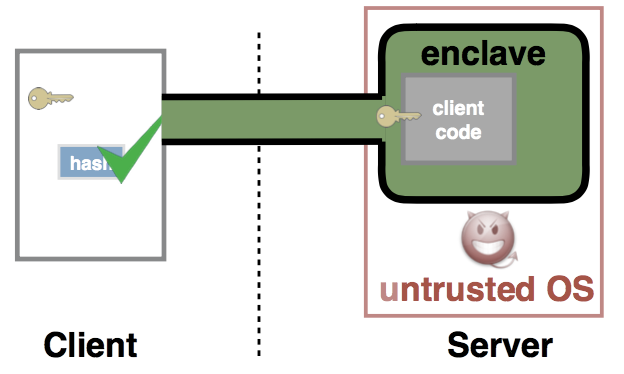
\includegraphics[scale=0.3]{images/uos}
%	\caption{Overview of remote attestation available in Intel SGX \cite{wang2017}.}
%	\label{fig:uos}
%\end{figure}

\begin{figure}
	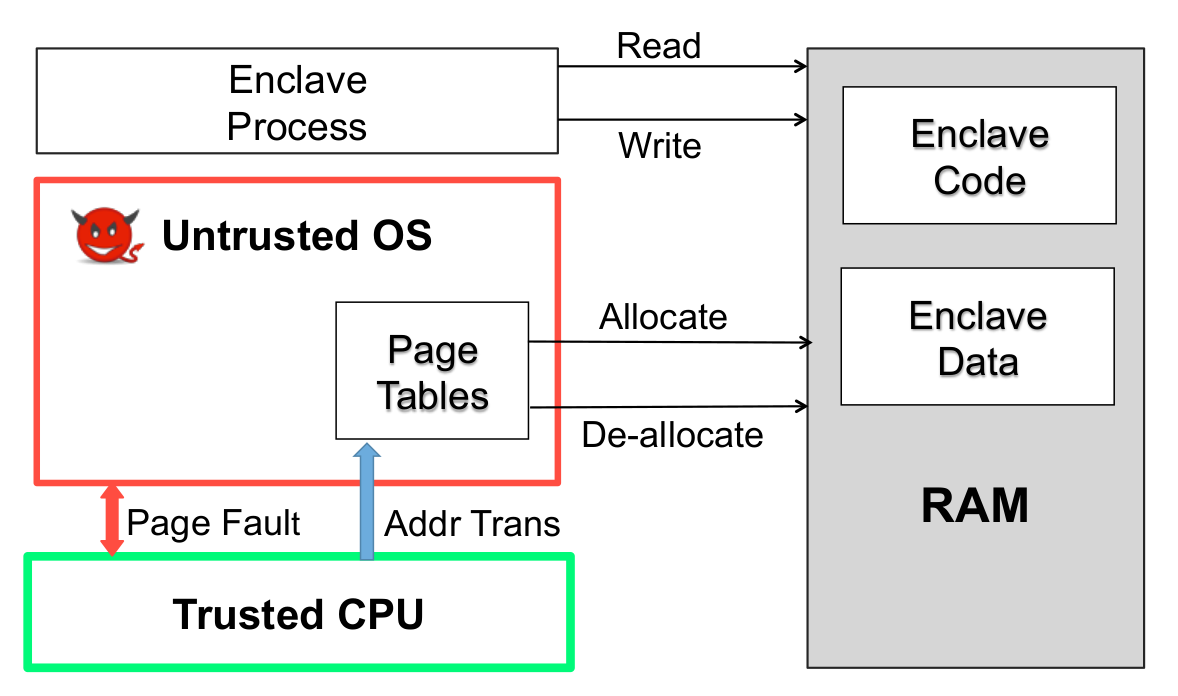
\includegraphics[scale=0.2]{images/uos1}
	\caption{Problem Setting. Process executing in an enclave on untrusted OS \cite{pigeonhole}.}
	\label{fig:uos}
\end{figure}

\subsection{Intel TSX}
One of the technologies that has attracted a great attention for making benefit in defense against side-channel attacks is Intel TSX \cite{tsx}. This technology has been introduced by Intel since Haswell micro-architecture \cite{haswell} for critical sections management and monitoring serialization. Intel TSX provides two frameworks to add transaction support to the processor. Both frameworks introduce new instructions for region specification, backward compatibility, and flexibility \cite{tsx}. One of them is RTM (Restricted Transactional Memory) \cite{rtm} which has been used by previous research like T-SGX \cite{tsgx} to isolate instructions and Cloak \cite{cloak} to pin sensitive code and data to the caches which are not supported by current hardware instructions.

\begin{figure}
	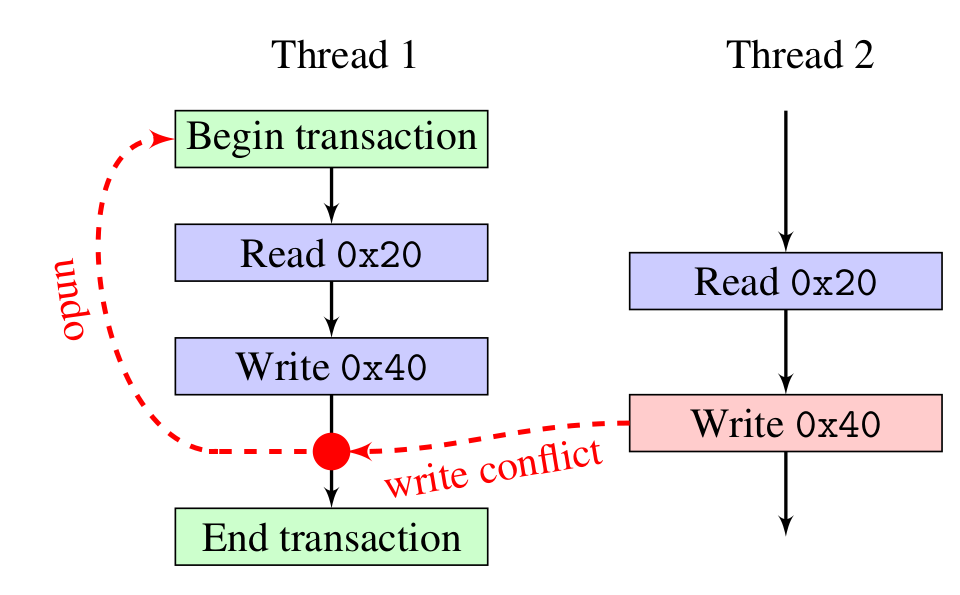
\includegraphics[scale=0.2]{images/rtm}
	\caption{HTM ensures that no concurrent modifications influence the transaction, either by preserving the old value or by aborting and reverting the transaction. \cite{cloak}.}
	\label{fig:rtm}
\end{figure}


\section{Attacks}
In this section, we introduce and discuss the attacks which use side-channel and focus on summarizing the methods and points of attack.

\subsection{Attack Model}
In our attack scenario, the enclave is protected by Intel SGX, so no one except the main program running inside enclave has the key to access it. The operating system kernel which runs on top of a hypervisor can view and manage tasks queue, exceptions and interrupts. The hypervisor kernel is also capable of viewing data transfer between memories and caches while Intel SGX prevents it from accessing the enclave data. It is considered that other tenants executing on the same hypervisor are not able to control the resources assigned to the main machine by the hypervisor.

\subsection{Points of Attack}
Several caveats with SGX architecture have been studied to be points for launching attacks against the enclave.

TLB, as an address translation cache, can be one point of attack. While TLB is shared between enclave and non-enclave programs when hyperthreading is enabled, it can create side-channels which can be used for retrieving useful information \cite{leakycauldron}.

Also, during AEX (Asynchronous EXit), TLB and paging-structure caches will be flushed and let the adversary know the flushed entries at context switch \cite{leakycauldron}.

Another point of attack is the use of page table entry flags. The accessed and dirty bits which are set and unset for page table entries upon accesses and modifications are used for launching attacks. So, the code in non-enclave mode can observe page-table updates and the memory write pattern to recover useful data \cite{leakycauldron,stealthy}.

Other than TLBs, CPU caches are shared between the enclave and non-enclave code resulting in the possibility of cache side-channel attacks \cite{leakycauldron}.

\subsection{Prime+Probe}
Prime+Probe is composed of two stages. Considering an L1 cache of 64 sets, each containing 8 cache lines which are each 64 bytes, in the prime stage, the attacker executes conflicting cache lines to make page fault possible for the victim who branches on a secret (Alg. \ref{alg:one}). In the probe step, the attacker executes all the cache lines and measures the execution time of each, and if a cache line execution takes longer, it can be revealed that the secret has been zero \cite{primeprobe1,primeprobe2,cloak} (Fig. \ref{fig:ppone}, \ref{fig:pptwo}).

\begin{algorithm}[t]
	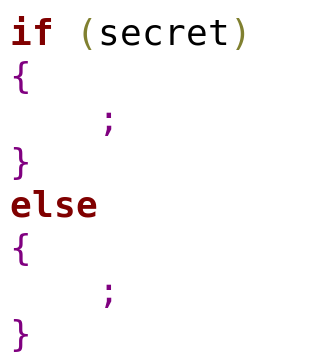
\includegraphics[scale=0.25]{images/alg}
	%	\SetAlgoNoLine
	%	if ($secret$)
	%	\\\{\\
	%	\tab ;\\
	%	\}\\
	%	else\\
	%	\{\\
	%	\tab;\\
	%	\}
	\caption{Prime+Probe branching side-channel sample code \cite{stealthy,cloak}}
	\label{alg:one}
\end{algorithm}

\begin{figure}
	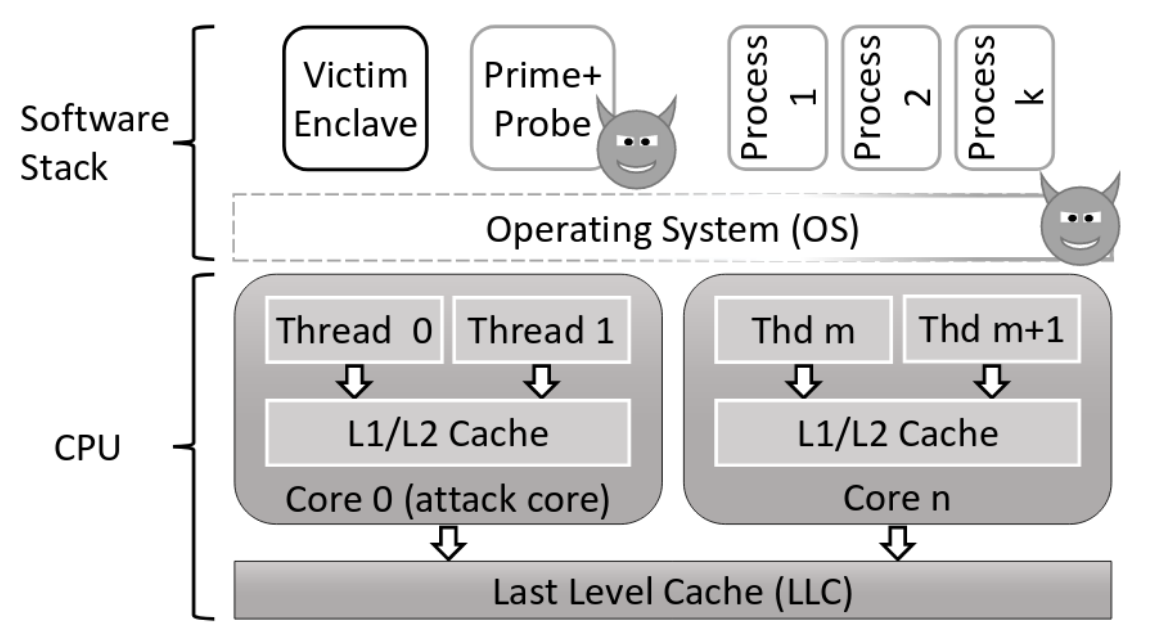
\includegraphics[scale=0.2]{images/pp1}
	\caption{A high-level view of the Prime+Probe attack; victim and attacker’s Prime+Probe code run in parallel on a dedicated core. The malicious OS  ensures  that  no  other  code shares that core to minimize noise \cite{brasser2017software}.}
	\label{fig:ppone}
\end{figure}
\begin{figure}
	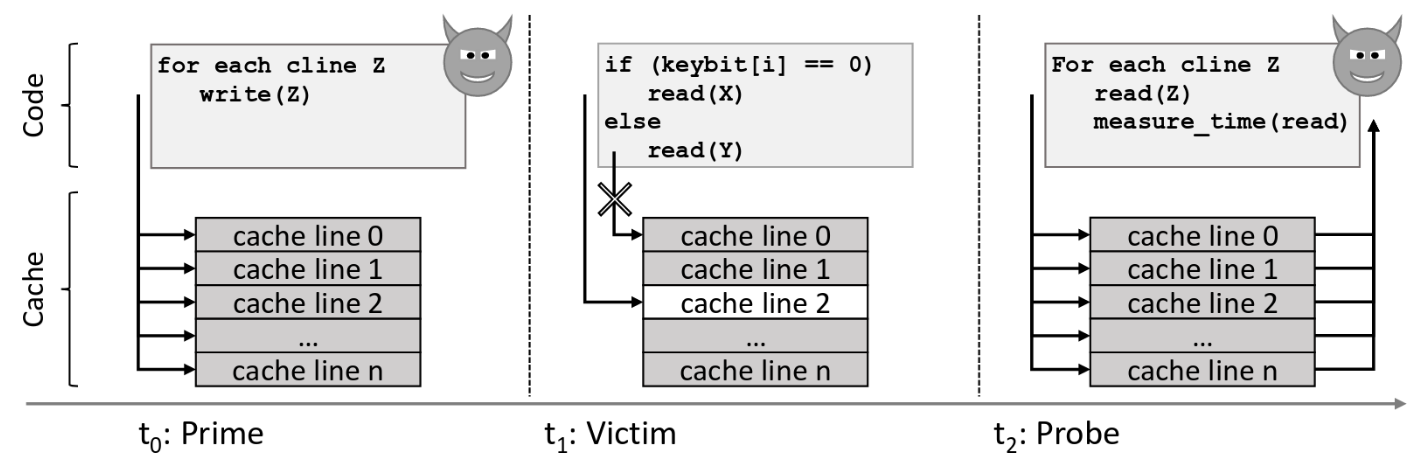
\includegraphics[scale=0.2]{images/pp2}
	\caption{A detailed view of Prime+Probe side-channel attack; first the attacker primes the cache, next the victim executes and occupies some of the cache, then the attacker identifies which cache lines have been used by the victim. This information allows the attacker to recover secret data in use by the victim process \cite{brasser2017software}.}
	\label{fig:pptwo}
\end{figure}

\subsection{Flush+Reload}
By making use of page sharing between enclave and non-enclave code, the attacker can find out if a certain page is removed from the cache. More precisely, the attacker flushes the target memory line from the cache and waits for the victim to access it. The wait time can be fixed to either a random value or a value that is experimented to be good for the attack success. Then, the attacker requests to access the page and measures the time it takes for the page to be fetched. Judging based on the time, the attacker can say if the page is already cached or fetched from the memory. In the case that it takes longer than a certain amount of time for the page to be retrieved, the attacker can conclude that it has not been fetched or touched by the victim \cite{flushreload}.

\begin{figure}
	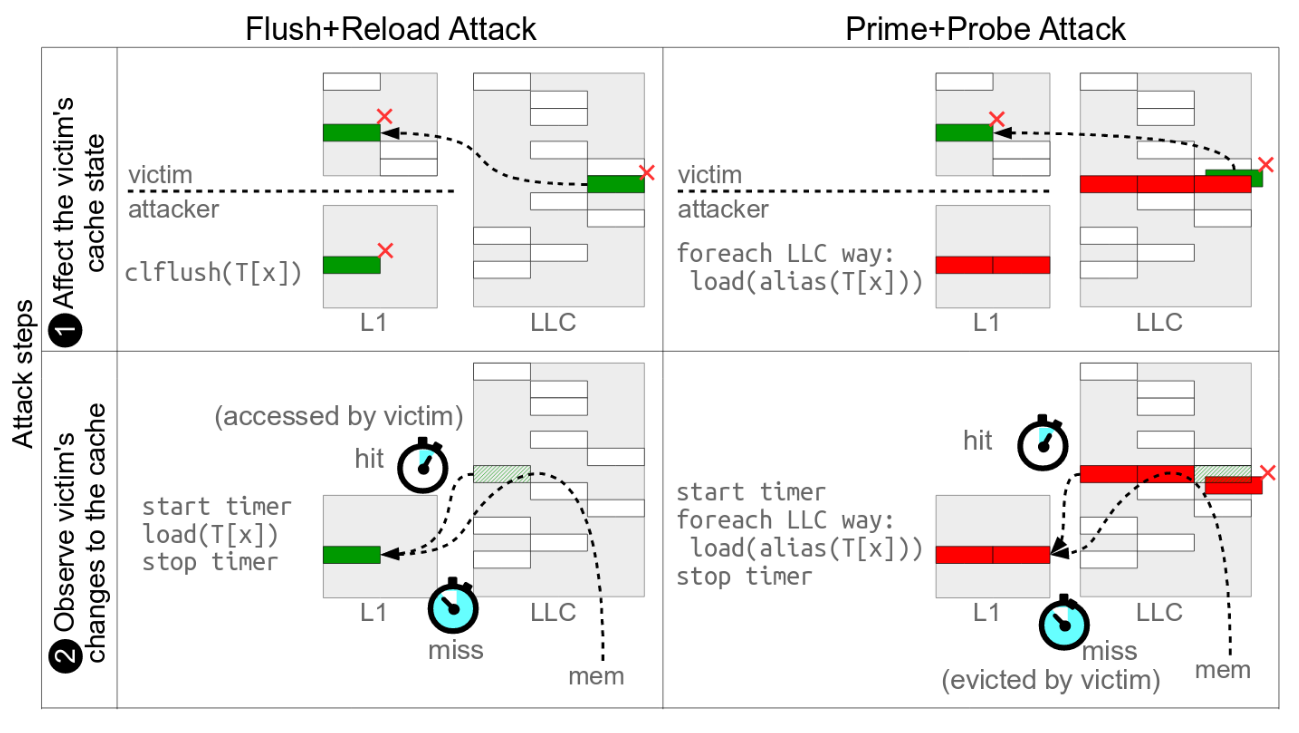
\includegraphics[scale=0.28]{images/ppfr}
	\caption{Prime+Probe vs Flush+Reload Attacks \cite{kayaalp2016high}.}
	\label{fig:ppfr}
\end{figure}

\subsection{Stealthy Page Table-Based Attacks}
Regarding the emerging of various page-fault based side-channel attacks, it is important to come out with a method for retrieving information without causing page-faults. Intended page-faults are possible to protect, and also cause a lot of overhead which leads to attack detection.

Van Bulck et al. \cite{stealthy} have confirmed that accessed and dirty flags are set and unset for page table entries in both enclave mode and non-enclave mode. Monitoring these attacks can lead to page-fault detection on protected memory region without the need to produce intended page-faults. Suppose a program is being executed in the enclave which branches based on a secret. If the branch occurs one page will be retrieved and thus its accessed flag will be set, otherwise the same happens for another page. By observing the accessed bit for these two page tables, the secret is revealed. Doing this sequentially can reveal all the secrets \cite{stealthy}.


\subsection{Sneaky Page-Monitoring Attacks}
Wang et al. \cite{leakycauldron} introduce three kinds of attacks for monitoring page-table entries with the consideration of the performance slowdown caused by producing intentional page-faults. In the case that a page-fault occurs for each memory access by the victim, the number of page-faults and performance slowdown can be a point for attack detection.
\subsubsection{Accessed flags monitoring}
Accessed and dirty flags of page table entries, as discussed earlier, can be used to trigger attacks without causing page-faults. In this attack, the attacker monitors the set-unset pattern of the flags for page table entries and recovers information about the program running inside the enclave and encrypted data which is being accessed in the protected memory. A problem with this attack is that after address translations are cached in the TLB, the flags are no longer updated in the page-table, but are updated in the TLB. Thus, it is needed to force the victim to walk its page-tables in order for the flags to be updated. In this attack, the attacker flushes the TLB by initiating an inter-processor interrupt which causes TLB shootdown. Thus, the flags will need to be updated in the page-table before being cached in the TLB \cite{leakycauldron,stealthy}.
\subsubsection{Timing enhancement}
The high number of accesses to a page-table entry for a certain input, can result in lots of interrupt requests in accessed flags monitoring attack which can be detected by monitoring interrupt requests by the victim. To prevent this, by finding out two pages which are accessed by the victim repetitively and measuring the time between these two page accesses, the input can be recovered. Thus, instead of multiple interrupts, one interrupt after each cycle is enough for clearing the TLB and successful attack \cite{leakycauldron,stealthy}.
\subsubsection{TLB flushing through Hyperthreading}
To further remove the interrupts which are needed by the two aforementioned attacks, it is possible to make use of the fact that the TLB is shared between two threads which are being executed on the same core. Thus, by running the attacker program in the same core with the victim program, it is possible to invalidate TLB entries outside the enclave without interrupt requests \cite{leakycauldron,stealthy}.

\subsection{DRAMA Attacks}
With caching disabled to prevent cache-based side-channel attacks, the attacker allocates two memory lines in the same memory segment which map to different virtual addresses but have common physical addresses. Then the attacker starts to regularly access one of the memory lines. In case the victim accesses the other memory line, a row conflict will cause the next fetch of the attacker to take more time. By measuring these times the attacker can recover the sensitive memory accesses by the victim \cite{leakycauldron,drama}.

\subsection{Cache-DRAM Attacks}
Using two threads for launching the Prime+Probe attack \cite{primeprobe1, primeprobe2} and DRAMA attacks \cite{drama} together, Prime+Probe can cause conflicts in the cache which leads to fetching the data from DRAM, making DRAMA attack possible in the case caching is disabled. Therefore, by launching this attack, the slowdown caused by disabling cache in DRAMA attacks is avoided \cite{leakycauldron} (Fig. \ref{fig:cachedram}).

\begin{figure}
	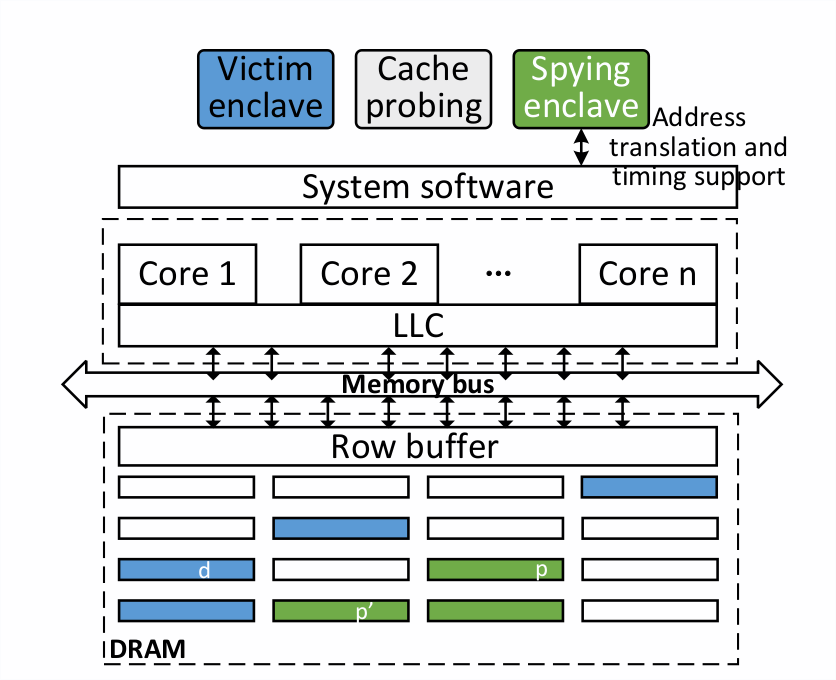
\includegraphics[scale=0.3]{images/cachedram}
	\caption{Cache-DRAM attack \cite{kayaalp2016high}.}
	\label{fig:cachedram}
\end{figure}

\subsection{Flush+Flush}
Using the \emph{clflush} instruction, it is possible to flush a cache line and if the cache line is already empty, the instruction will abort. Considering that the abort takes less time than the flush, it is possible to use this delay to recover information about the content of the cache. By observing the existence of data inside the cache line, it is possible to find out which memory address has been accessed by the victim. By running the \emph{clflush} instruction repetitively and measuring its execution time, the attacker retrieves this information \cite{flushflush}.

\section{Defenses}
We discuss the research that has been done on protecting the enclave against the mentioned side-channel attacks and their effectiveness. Some research study on preventing the attack from being performed and some intend to defend the enclave against attacks and block them.

\subsection{Attack Detection}%{Déjà Vu}
One of the methods that lead to the prevention and defense against the attacks is to detect the attack and stop executing completely, or while the attack is in action.

Chen et al. \cite{dejavu} embed a clock inside the enclave and use Intel TSX for detecting any interrupt to it. When the execution time of the program inside the enclave exceeds a fixed amount of time as the threshold, it is considered that the code has been interrupted by some external factor and an AEX (asynchronous enclave exit) will be detected. The implemented clock should be hidden from the OS in terms of reading and modification and it should not go backward in time under any condition. These can be assured by implementation inside SGX enclave. Also, the clock should not be stopped or interrupted by the OS which is solved by using TSX. For protecting the clock to be read by the OS, a random value will be generated in a transaction and will be added to the global timer variable. This will run in a thread parallel to the main program inside the enclave (Fig. \ref{fig:dejavu}). The threshold delay needs to be approximated by training the system with AEX-free execution time and minimum delay of an AEX execution.

\begin{figure}
	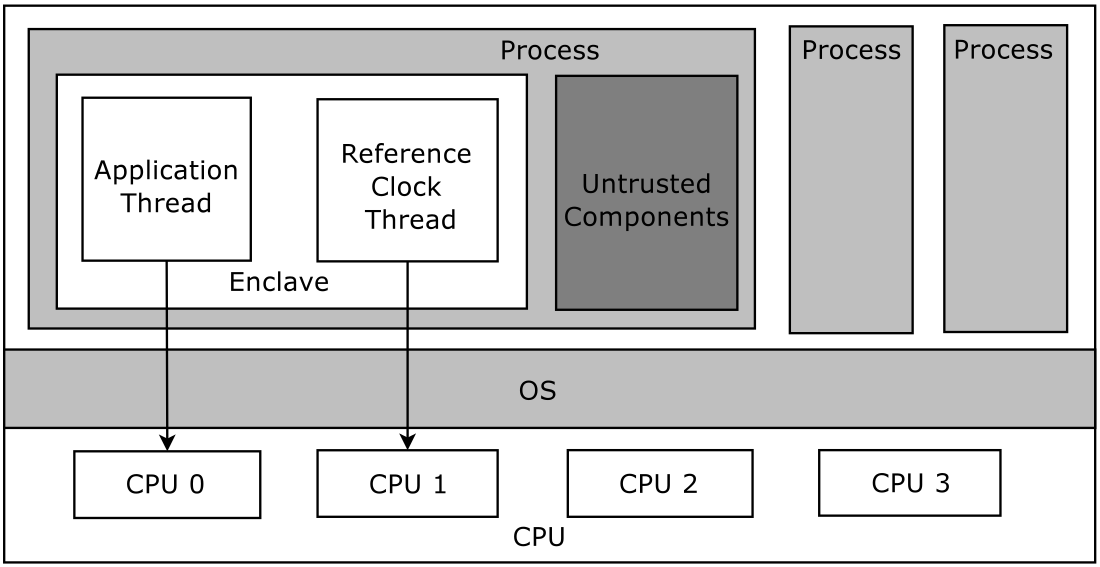
\includegraphics[scale=0.2]{images/dejavu}
	\caption{System architecture of Déjà Vu. Blocks in gray are untrusted, which include the untrusted components of the processes and the entire OS kernel \cite{dejavu}.}
	\label{fig:dejavu}
\end{figure}

Shinde et al. \cite{pigeonhole} conduct a statistical study on the percent of leakage, vulnerability, possibility and effectiveness of page-fault based attacks which they call pigeonhole attacks. Then, they consider the possible ways of eliminating page-fault side-channels. More precisely, they define pigeonhole attack as an attack that is performed when a page table walk is done. Moving data between the physical and virtual memory from different pages sequentially causes page-faults on every single page when the virtual memory is already full, holding all the other pages. When the first page is fetched, the next page will be removed from the page table and when the next page is to be fetched, a page-fault will occur. Based on the fact that the malicious OS cannot differentiate accesses which are occurred in a single page, they claim that by mapping all the input dependent data into a single page, the program will access the same pattern of the pages independent of the input and makes it page-fault oblivious. The page containing the input dependent data is called data staging page and the one containing the code is called code staging page. By creating a decision tree of the program instructions, it is understood that in each stage of the program which is being executed, there is a page-fault sequence dependent on the data, which can be mapped to a staging page. So, for each stage, one staging page is considered. This technique will create a high overhead, thus, the research extends to optimizing the implemented method by eliminating copy operations which is done by skipping read-only data save, merging small data blocks into single pages to reduce the number of fetches, merging levels of execution and reducing the number of stages, removing the mux based on the input to reduce the possibility of branch conditions, and removing the dependence of code on the data (Ex. CAS obliviousness).

Shih et al. \cite{tsgx} make use of Intel transactional memory technology to isolate enclave code from interrupts caused by intentional page-fault based side-channel attacks performed by a privileged OS. They improve the design by dividing the code into micro blocks to prevent abortions, because transactions are not designed to run long programs.


\subsection{Attack Prevention}%{Cache-based attacks}%cloak
It is known that in a multicore system, there are three levels of cache: L3 is shared between all physical cores, L2 is shared between each core's threads and L1 shares data and code separately between the hyperthreads. In a typical environment, it is not visible to the enclave program running in one thread, what is being run in the other thread on the same core. So, if the other hyperthread is trusted (assuming there are two hyperthreads running in each core) it is only needed to care about the L3 cache. In the SGX environment, the hyperthreads cannot trust each other, thus, L2 and L1 caches are also of importance when it comes to the case of cache side-channel attacks because attacks like Prime+Probe will be possible in this case \cite{cloak}.

The basic approach to confront cache-based side-channel attacks including Prime+Probe and eliminate the leakage is to pin sensitive code and data into caches so no conflict and cache-miss be possible, but it is impossible to pin data into caches in the current hardware/software environment. So, there is a need to introduce a hack for indirectly doing this which has been implemented using Intel TSX by Gruss et al. \cite{cloak}.

By studying the in-depth architecture of TSX instructions, it is found that TSX uses a write set and a read set and interrupts to these sets cause the transaction to abort. The write set is always the 32kb L1 and the read set is the 8mb sized L3. So, if a cache line in L1 is modified and made dirty, the transaction aborts. The same happens when some cache line in L3 is removed due to a conflict. Also, it is observed that code, which is read-only, can only be a part of the read set L1. This has the benefit of detecting external code evictions by other cores which share the same L3 cache \cite{cloak}.

After explaining the indirect effect of using TSX for pinning data to cache, it is needed to load the data and code into the cache inside a TSX transaction. After that, each cache conflict which leads to making cache access pattern to be visible will cause the transaction to abort. So, the sensitive code and data will be preloaded and the program will start to run inside the transaction. Then, the victim does not experience cache misses and there is nothing for the attacker to measure, so the enclave is protected against the malicious OS \cite{cloak}.

\begin{algorithm}[t]
	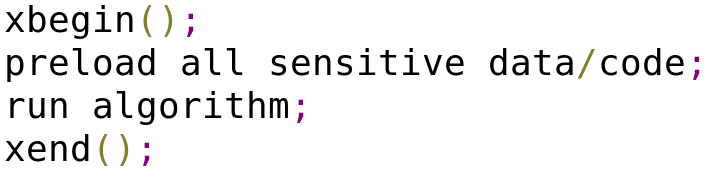
\includegraphics[scale=0.25]{images/cloakcode}
	\caption{Cloak sample code \cite{cloak}}
	\label{alg:cloak}
\end{algorithm}

For preloading, if the attacker targets L1, the code should be preloaded into L1-I by execution. Also, all the data should be loaded into the write set. For the attackers targeting L3, code and read-only data should be loaded into read set, while the data which will possibly be touched again should be loaded into the write set \cite{cloak}.

Seo et al. \cite{sgxshield} study address space layout randomization (ASLR) which is used in traditional systems for defending the memory against corruption attacks, but SGX does not make benefit of it. They present a new ASLR scheme for SGX systems and study the new challenges which come with it. Including the problem of small randomization entropy which is a result of limited physical and enclave memory and makes brute force attacks possible. Also, the inability of runtime page permission change makes the enclave vulnerable to code injection attacks due to conflicts with ASLR which is addressed by implementing a software-based RWX permission set.

\begin{figure}
	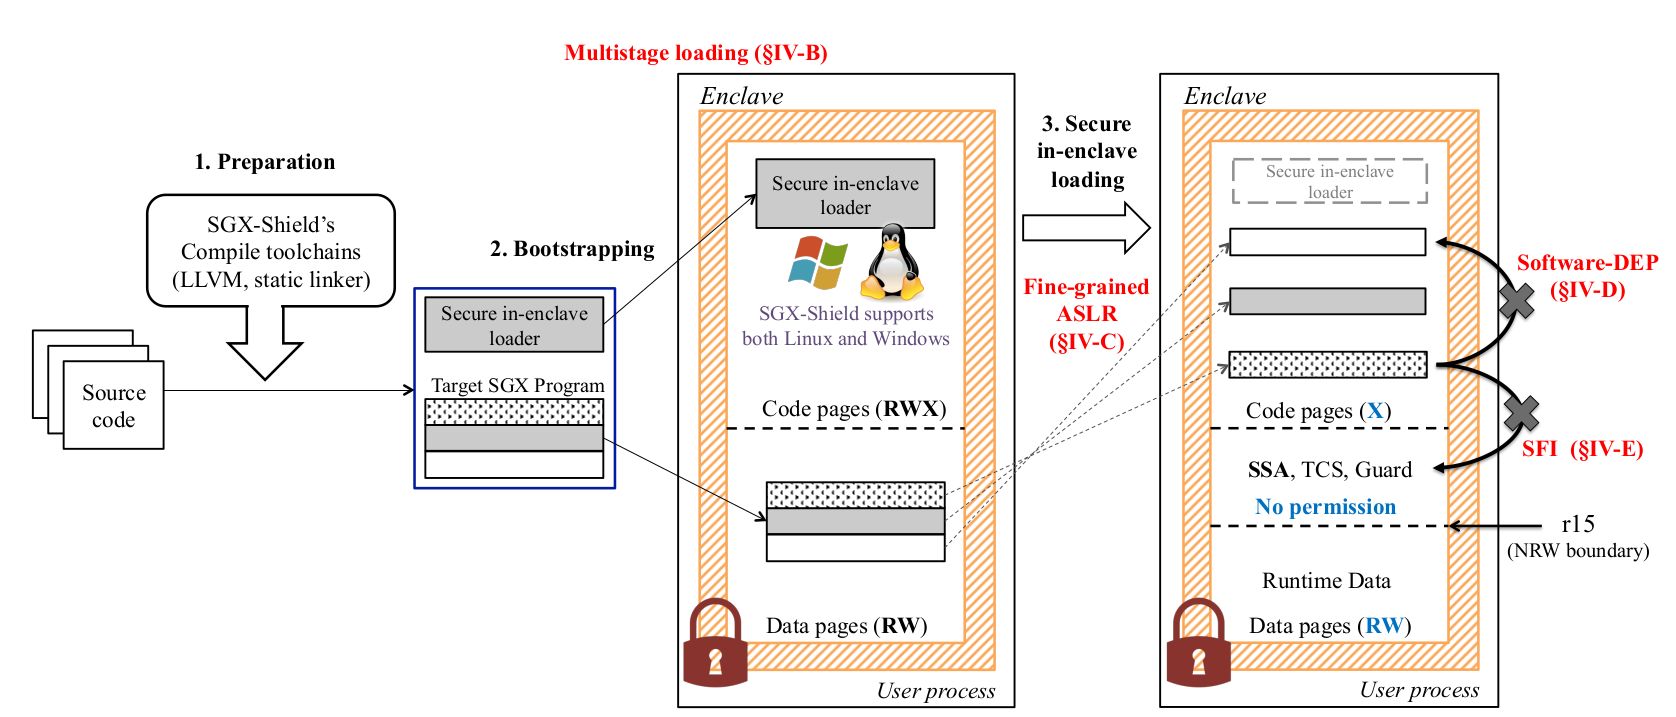
\includegraphics[scale=0.2]{images/sgxshield}
	\caption{Overall workflow of SGX-Shield: 1) the preparation phase builds a SGX binary from the target program’s source code; 2) the bootstrapping phase loads the secure in-enclave loader into code pages and the target SGX program into data pages; and 3) the secure in-enclave loading phase finally loads the target SGX program \cite{sgxshield}.}
	\label{fig:sgxshield}
\end{figure}

Sasy et al. \cite{zerotrace} implement a block level memory controller as a new library combining ORAM \cite{oram1,oram2,oram3} and Intel SGX while mitigating the disadvantages of these technologies and protects the enclave from software-based side-channel attacks meanwhile optimizing the performance.

Brasser et al. \cite{drsgx} propose data location randomization as a new approach for defending enclave side-channel attacks by designing and implementing a compiler based tool to shuffle the in-enclave data locations at the granularity of cache lines.

\section{Analysis}
Cloak \cite{cloak} has achieved significant protection against cache-based side-channel attacks. However, there will still be some leakage remaining which this research does not handle. Overall execution time can leak information. Also, aborts do not cause the concurrent memory accesses to be canceled. Branch predictor is influenced due to the cache pinning and other micro-architecture effects can be possible due to the modifications to the execution behavior. On the other hand, the introduction of a new software-based way for pinning data into cache lines and making use of transactions for this purpose is a novel idea that opens new ways for future research in several areas. There is also an opportunity for later research on optimization and performance improvement and architectural study for reducing faults.

T-SGX \cite{tsgx} protects the enclave against page-fault based side-channel attacks, but at the same time, attacks which are based on monitoring accessed and dirty bits of the data are not detected by this method.

The problem with Deja Vu \cite{dejavu} is that it only considers enclave exits as points of attacks and possible attacks that may have been occurred during the execution which do not cause AEX have been excluded. So, attacks like B-SPM and HT-SPM (sneaky page monitoring attacks in general) which do not rely on AEX can still be effective \cite{leakycauldron}.

Overall, all the techniques based on using transactions to isolate the program from interrupts and immune them to page-faults, need an isolated executing environment which causes a single thread execution, low utilization, and high overhead.

Randomization, as studied in \cite{sgxshield} can be a leading point for research on possible defenses. However, it is used to implement an ASLR for SGX which is not lively randomized. Thus, the attacker can observe the random patterns of memory accesses for multiple times and infer an approximate access pattern which is helpful for launching attacks \cite{leakycauldron}. Also, the implementation is not evaluated against brute force attacks, so, the amount of introduced entropy cannot be verified to be effective.

The work done by Shinde et al. \cite{pigeonhole} does not take cache-based side-channel attacks into account. The idea of loading all the sensitive data into the same pages can still leak information using cache and TLB side channels \cite{leakycauldron}.

The bottom line is that none of the proposed methods can completely defend the enclave against the possible side-channel attacks. Page-fault detection cannot protect the enclave since page accesses can be learned without causing page faults. It is not even needed to interrupt the enclave for reading the TLB. Thus, any solid defense method needs to either remove all the branches and conditional code/data from the program or find a way to reliably pin specific data/pages to the cache and therefore TLB.

\begin{comment}

\section{Future Research}
The past researches that have been studied in this report, open new spaces for continuing research to achieve better results in terms of security and performance. We discuss some ideas which can be the starting point for future research in this section.

\subsection{Noise Generation Using a Helper Thread}
\subsubsection{Scenario 1}
We know that the shared TLB by multiple hyperthreads running on a single core of CPU can be cleared or modified by the program running in one of the hyperthreads. This can be a method for attacking the other hyperthreads which may be executing a program inside an enclave. We may use a parallel thread to the enclave thread to help defending it. There is a chance that the page faults initiated by the enclave can be randomly affected by the helper thread. Thus, we can execute a program of random instructions fetching random data in a hyperthread parallel to the enclave. The frequency of memory accesses in the helper thread and the balance between overhead and security is subject to research. By generating random noise, the helper thread causes fake page faults which can make the page fault frequency and patterns of the sensitive program execution inside the enclave to be hidden. However, in this case, the malicious OS can complete the faults caused by the helper thread to cause a page table walk by the main thread and recover the data. Also, a differential analysis to recover sensitive repeated non-random accesses can result in a failure for this method.

\subsubsection{Scenario 2}
A fix can be making the threads share the same memory slot. This is possible by creating an SGX thread inside the enclave program. The helper thread will run random instructions which randomizes access patterns based on random inputs while the main thread runs the main program. It will not be visible to the malicious OS which program is causing the page faults and the behavior of the helper thread program changes frequently. But a malicious OS is responsible for thread scheduling and by detecting, or simply guessing the helper thread, can postpone or suspend its execution using the thread scheduler unit. The possibility of helper thread identification can be minimized by creating unlimited helper threads but this is not efficient. If the program running inside the enclave has parallel behavior and can be multithreaded itself, two threads can run simultaneously cooperating while generating noise at the same time. Also, it is possible for the two threads to run the same program while generating noises. But a possible attack is that the OS can first run thread 1 multiple times to see which page faults are occurring multiple times and then identify random noisy page faults.

\subsubsection{Scenario 3}
In scenario 1, if a second helper thread exists, we should identify if it is suspended from running by the malicious kernel, then we know we are being attacked. The helper thread should create the permission for the main thread to continue running.

\subsubsection{Scenario 4}
The main thread can wait for the helper thread to start. The helper thread starts accessing random addresses inside enclave inside a transaction. The main thread also runs inside a transaction. Any page fault inside the enclave region will cause both transactions to abort. Also, any context switch on the helper thread, for the malicious kernel to stop it from executing, will cause transaction abort. This will solve the problem with T-SGX \cite{tsgx}. Accessed bits will still be set randomly, while page faults are being detected. So, neither page faults nor accessed bits observation can be useful for recovering information. The frequency of the accesses by the main program can be a point for detecting noises, while noises occur less because of their randomness. This can be addressed by introducing a random repeating pattern by the helper thread other than randomly generated noise. It is possible for the helper thread to signal the main thread to stop executing if a page fault occurs. So there is no need for the main thread to run as a transaction. This solves the starvation problem that is addressed by micro transactions in T-SGX \cite{tsgx}.

\subsubsection{Scenario 5}
After all, it is still visible to the malicious privileged OS that what process accesses the memory and causes the page faults. So, the idea is subject to more research and improvement.

\subsection{Parallel Data Fetch}
Array access obliviousness can be achieved by using a single SIMD instruction to gather multiple addresses from memory. This will help achieve good performance and gather multiple values which are not visible to the adversary which one is going to be used. Any page fault and accessed bit modification will be done for all the accessed pages. The same happens for modified bits when writing to the memory using a scatter SIMD instruction. Meanwhile, the page fault access pattern is still visible because same offsets of memory are always read when gathering with a single target value multiple times. This can be prevented by randomly changing the offset.

\subsection{Data Shuffling}
Data shuffling is one of the major methods for causing entropy and irregularity that lead to different behavior by the program and make the patterns disordered, thus making it harder for the attacker to tamper with the data flow and patterns. Several works like \cite{melbourne} have been done on obliviously shuffling the data to provide security to cloud environment.

We make use of data shuffling for increasing the entropy of the data which is passed to our program. The programmer calls a function to read the data sequentially inside enclave and shuffling it using a random permutation. For a data with size $n$, a permutation can be generated by rendering a list of values $ 1..n $ and shuffling it. So, the permutation creation needs an oblivious and secure shuffling algorithm itself. We can generate $n$ random values inside the enclave which basically allows repeated values, then obliviously sort the data based on the random values. We must note that this permutation that allows containing repeated values can decrease the accuracy of our shuffling algorithm.

\subsection{TLB Shootdown}
TLB shootdown is one of the usable methods for SPM attacks \cite{leakycauldron,stealthy}. When an address mapping is cached in TLB, the accessed bit will not be set for each access, hiding the accessed bits reset pattern from the adversary but the attacker can make the flags updated by clearing the TLB and causing the page address mapping to be accessed again. This can be done by interrupting the CPU frequently and causing a TLB shootdown. Whenever the processor exits from enclave execution due to an interrupt, a TLB shootdown is performed to clear the TLB data that was being used by the enclave program. The attacker can achieve this by toggling an interprocess interrupt (IPI) to cause an AEX (Enclave Exit) \cite{stealthy}.

We defend this attack by shooting down the TLB after the execution of the sensitive instruction inside enclave. Any interrupt will cause transaction abort and program termination. And any flag updates is flushed by the enclave program. Thus, the attacker cannot read the bits frequently to infer the pattern and fails to launch an HT-SPM attack. In another word, the attacker will not be able to access TLB entries for the enclave thread. But the attacker can still access page-table which needs an interrupt that leads to transaction abortion and attack detection.
\end{comment}


\section{Conclusion}
In this report, we studied various kinds of attacks proposed by the past research and also reviewed the defenses in terms of their technique, security, and performance, also analyzed their effectiveness. While several attacks can be practical to a good extent, there are still points of attacks and there is still space for security and performance improvements. Finally, the area is subject to further extensive research according to various unknown attacks which emerge every day.

\begin{acks}
	
	This work has been done for the fulfillment of Ph.D. candidacy as qualification examination 2 (QE-2) at Syracuse University Department of Engineering and Computer Science for Computer and Information Science and Technology (CISE) program.
	
	%The research has been advised by Dr. Yuzhe Tang and Dr. Steve Chapin at Syracuse University.
	
\end{acks}

% Bibliography
\bibliographystyle{ACM-Reference-Format}
\bibliography{bibliography}